\documentclass[12pt, a4paper, dvipdfmx]{book}
\usepackage{listings,jlisting}
\usepackage{graphicx}
\usepackage{pxrubrica}
\usepackage{here}
\usepackage[dvipsnames]{xcolor}
\lstset{
basicstyle={\ttfamily},
identifierstyle={\small},
commentstyle={\color{OliveGreen}},
keywordstyle={\small\bfseries\color{RedViolet}},
ndkeywordstyle={\small},
stringstyle={\small\ttfamily\color{red}},
frame={tb},
breaklines=true,
columns=[l]{fullflexible},
numbers=left,
xrightmargin=0zw,
xleftmargin=3zw,
numberstyle={\scriptsize},
stepnumber=1,
numbersep=1zw,
lineskip=-0.5ex
}
\renewcommand{\familydefault}{\sfdefault}
\title{テトリス on Pygame}
\author{Swimmy高田馬場校}
\begin{document}
\maketitle
\tableofcontents
\chapter{はじめに}
わからないことがあっても気にしないでください。これから学ぶオブジェクト指向は本来大学の専門科目にあたります。
今も活発に研究が行われている分野ですし、今後10年で大きく変わる可能性もあります。
この本でおすすめしていることも、将来的には\ruby[g]{アンチパターン}{やってはいけない設計}と言われているかもしれません。
今自分はプログラミング言語の最前線を学んでいるんだなあと思って楽しんでくれれば嬉しいです。

\chapter{今まで通りに作る}
\section{いつも通り作ってみよう}
ヘビゲームと同じように、今までのように作ってみましょう。
\lstinputlisting[title={今までのような作り方}, language=Python]{chapter2/tetris.py}
\newpage
\subsubsection{実行結果}
ここまでできたら、次の章に進んでください。実行結果も載せてあるので比べてみてください。
\begin{figure}[h]
  \centering
  % 824x1600
  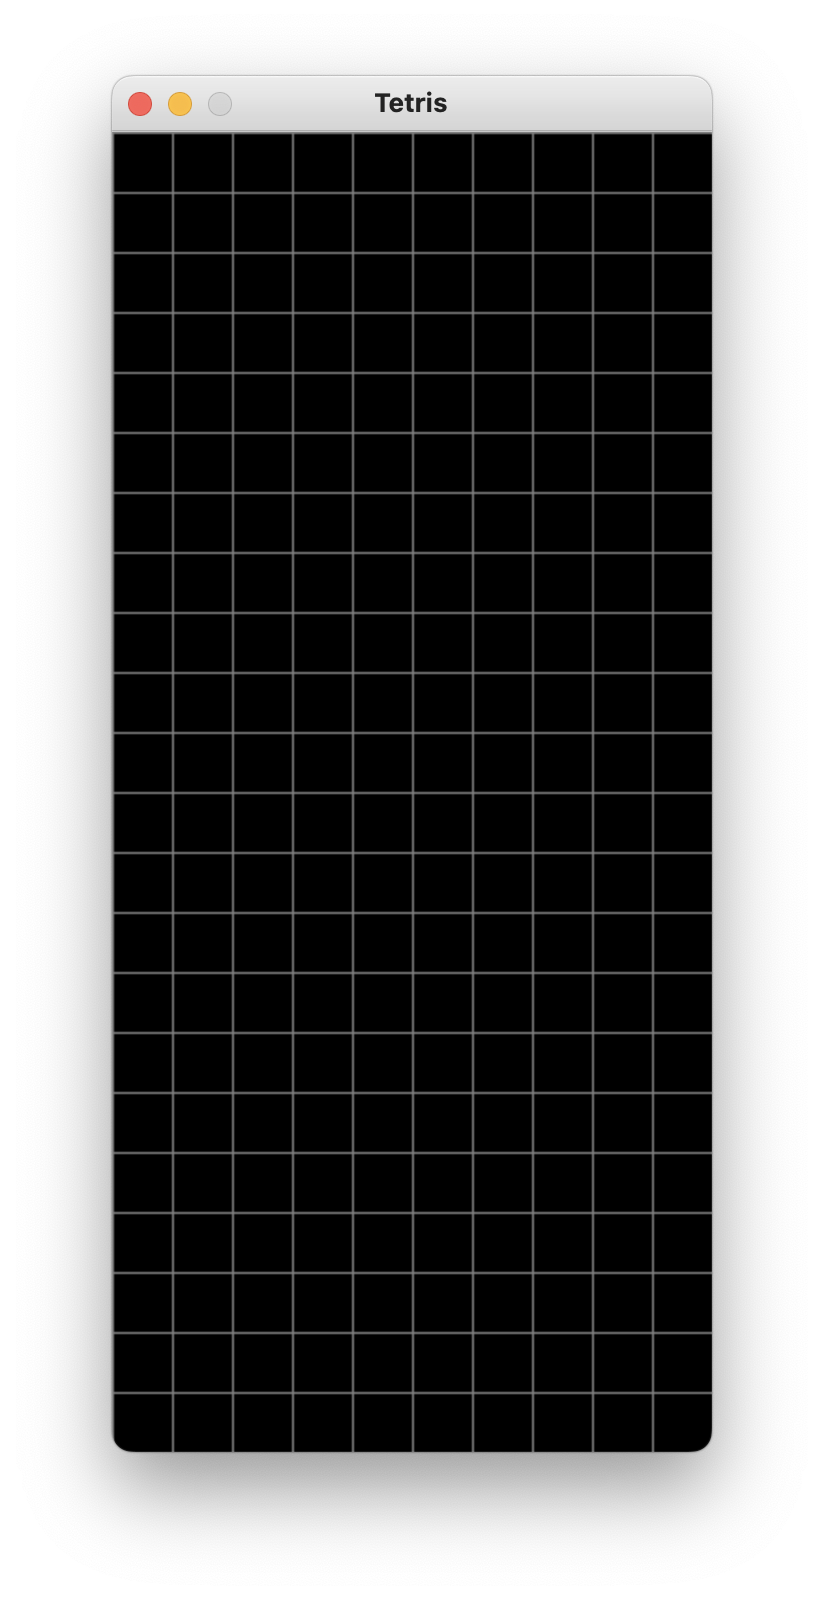
\includegraphics[height=15cm, natwidth=824,natheight=1600]{TetrisCH1_1.png}
  \caption{テトリスの実行結果}
\end{figure}

\chapter{オブジェクト指向プログラミングへ}
\section{オブジェクト指向プログラミング}
\subsubsection{プログラミング言語界の主人公的存在、オブジェクト指向}
今まで私たちは「変数」、「関数」を用いてプログラムを作ってきました。
\begin{lstlisting}[caption=復習,label=sample, language=Python]
# 変数の作り方
名前 = "ATAI"

# 関数の作り方
def 関数名():
    # その時にすることを書く
    print("こんにちはよいお日和ですね")
\end{lstlisting}
変数はデータに名前をつけることで、関数は処理に名前をつけることでした\footnote{厳密には、変数とはデータの領域に名前をつけることです。}。
オブジェクト指向プログラミングは主に「クラス」という「プログラムそのものに名前をつけたもの」を構成することで
プログラムを作ります。クラスは「変数」と「関数」を持つことができます。つまり、どんなPythonファイルも一つのクラスにまとめることができます。
\section{クラスの作り方}
\subsection{クラスの作り方}
クラスは以下のように作ります。Pythonファイルの中で何個でも作ることができます
\footnote{しかし、みやすさの観点からクラスは1ファイルにつき2〜3個までにする人もいます。}。
\newpage
\begin{lstlisting}[caption=クラスの作り方,label=sample, language=Python]
class クラス名:
    ...
\end{lstlisting}
クラス名は作りたいクラスに応じて変えてください。...は省略しているわけではなく、
「後で書きます」というちゃんとしたPythonのプログラムです。

\subsection{クラスを変数に入れる}
クラスは設計図のようなもので、実際に使うには\textbf{作って変数に入れる}必要があります
\footnote{このような変数のことをインスタンスと呼んだりします。Pythonの場合、全ての変数は何かのインスタンスになるらしいです。}。
\begin{lstlisting}[caption=クラスを変数に入れる,label=sample, language=Python]
変数名 = クラス名()
\end{lstlisting}
\textbf{「クラスを作る」とは「クラス名()」と書くこと}です。作ったクラスは変数に入れないと
次の行には捨てられています
\footnote{捨てられていないこともあります。
  PythonはARCと世代別GCの二種類を持っているらしく、クラスに循環参照がある場合はGCにより時間差で捨てられます}。
なので、大体の場合は「変数名=クラス名()」と書くことが多いです。
カッコの中に何が入るかは、クラスによって異なります。後で説明します。

\subsubsection{関数と似てる?}
クラスは関数と似ている部分があります。関数は使う前になるべく関係ないところで「def 関数名():」と書いて「宣言」
\footnote{こういうものだよ、と決めること}しましたね。
\begin{lstlisting}[caption=関数の作り方,label=sample]
def 関数名():
  # 呼ばれた時にすることを書く
  ...
\end{lstlisting}
実際に使うときは、その場所で「関数名()」と書きましたね。
\begin{lstlisting}[caption=関数の呼び出し方,label=sample]
関数名() # 「呼ばれた時にすること」が実行される
\end{lstlisting}
カッコの中には何かが入ったり入らなかったりしますが、関数を使うときは「関数名()」と書きました。
似てますよね。プログラムが複雑になったときに
宣言と使う場所を分離することでプログラムをみやすくするという考え方です。

\section{クラスの中に変数を作る}
\subsection{クラスの中に変数を作る}
普通の変数の作り方と\textbf{ほぼ}同じです。
\begin{lstlisting}[caption=クラスの中に変数を作る,label=sample, language=Python]
class クラス名:
    def __init__(self):
        self.変数名 = 値
\end{lstlisting}
\_\_init\_\_関数は\textbf{クラスを作って変数に入れるときに自動で呼ばれます}。
変数を作って入れることもできますし、printを書くとクラスをつくるたびに表示されるようにすることもできます。
たとえば、教科書に「Mentorクラスを作って、中にageという変数を作る。ageには最初に20を入れる。」という文章があったら、
\begin{lstlisting}[caption=Mentorクラスの作り方,label=sample, language=Python]
class Mentor:
    def __init__(self):
        self.age = 20
\end{lstlisting}
こう書きましょう。\textbf{変数は一つだけでなく何個でも作れます}\footnote{パソコンの覚えられる量を超えない限り}。
さらに、「nameという変数を作って、先生の名前を入れてみよう」という文章があったら、
\begin{lstlisting}[caption=Mentorクラスの作り方,label=sample, language=Python]
class Mentor:
    def __init__(self):
        self.age = 20
        self.name = "先生の名前を入れる"
\end{lstlisting}
クラスはたくさん書くことで設計の仕方がわかっていくので、何度も書く→増やす→失敗する→改良するを繰り返して慣れていきましょう。

\subsection{クラスの変数の中身がわからない場合}
でも、先生の年齢がいつも20歳なのはちょっと変ですね。先生が常に20歳とは限りません。\textbf{クラスは設計図}なので設計段階ではわからない数値やデータもあります。
変数に入れる値がまだわからない時は、引数にすれば\textbf{実際に作る時まで先延ばし}にすることができます。
\begin{lstlisting}[caption=引数を使う場合,label=sample, language=Python]
class Mentor:
    def __init__(self, age, name):
        self.age = age
        self.name = name
\end{lstlisting}
このように書くことで、Mentorクラスを\textbf{作る時に年齢と名前を指定}することができます。
\begin{lstlisting}[caption=Mentorクラスの作り方,label=sample, language=Python]
# クラスを作る時に、年齢と名前を指定する
mentor1 = Mentor(20, "A先生")
\end{lstlisting}
30歳の先生を作る場合は、
\begin{lstlisting}[caption=Mentorクラスの作り方,label=sample, language=Python]
# クラスを作る時に、年齢と名前を指定する
mentor2 = Mentor(30, "B先生")
\end{lstlisting}
さっきのプログラム2つでは違う変数に同じクラスを作っていましたが、\textbf{クラスは設計図}なので、クラスを一度作っておくと、
別のデータで別の変数に似たデータを入れられます。設計図を元にカスタマイズしながら量産できるということです。
まだ便利さがわからないかもしれませんが、関数の引数とオブジェクト指向は
便利さがわかりづらいランキング1位と2位なのでここは少し我慢してください\footnote{作者の個人の感想です}。

\subsection{クラスの変数の中身を変更する}
クラスの変数の中身を変更するには、以下のように書きます。
\begin{lstlisting}[caption=クラスの変数の中身を変更する,label=sample, language=Python]
  mentor3 = Mentor(40, "C先生")
  mentor3.age = mentor3.age + 1
\end{lstlisting}
このように書くことで、mentor3の年齢を1歳増やすことができます。お誕生日おめでとうございます。
\subsection{クラスの変数を使う}
クラスの変数を使うには、以下のように書きます。
\begin{lstlisting}[caption=クラスの変数を使う,label=sample, language=Python]
  print(mentor3.age)
\end{lstlisting}
このように書くことで、mentor3の年齢を表示することができます
\footnote{このようなインスタンスに対して「.」を使ってアクセスする変数をインスタンス変数といいます。}。
普通の変数と同じように使えますね。変数の集まりがクラスと考える人たちもいます
\footnote{厳密には変数を一つに集める機能はストラクチャというものにもあるので、「クラス=変数の集まり」と覚えるのは不正確かもしれません}。

\newpage
\section{クラスの中に関数を作る}
関数の作り方も普通の関数の作り方と\textbf{ほぼ}同じです。
\begin{lstlisting}[caption=クラスの中に関数を作る,label=sample, language=Python]
class クラス名:
    def 関数名(self):
        ...
\end{lstlisting}
たとえば、教科書に「Carクラスを作って、runという関数を作る。run関数は「走ります」と表示する」という文章があったら、
\begin{lstlisting}[caption=Carクラスの作り方,label=sample, language=Python]
class Car:
    def run(self):
        print("走ります")
\end{lstlisting}
こう書きましょう。\textbf{関数も何個でも作れます}し、引数を使うこともできます。
\begin{lstlisting}[caption=引数を使う場合,label=sample, language=Python]
class Car:
    def run(self):
        print("走ります")
    def set_speed(self, speed):
        print("時速", speed, "kmで走ります")
\end{lstlisting}
テキストを読んでいて「クラスの中に〜」という文章があってよくわからない場合はこの章に戻ってきてください。
ちなみにCarクラスのrun関数を使うには、
\begin{lstlisting}[caption=Carクラスの使い方,label=sample, language=Python]
car = Car()
car.run()
\end{lstlisting}
と書きます。\textbf{クラスは設計図}なので、一度変数にしないと使えません。
\footnote{このように、インスタンスに「.」をつけて呼ぶことのできる関数をインスタンスメソッドと呼びます。}

\section{まとめ}
クラスは「変数」と「関数」\footnote{正確にはメソッドと呼ばれます。メソッド=手順、手続き}を中に持つことができます。クラスは設計図のようなもので、
実際に使うには変数に入れる必要があります。変数に入れるときは「変数名=クラス名()」のようにしますが、
クラスによってはカッコの中に何かを入れる必要があります。

\subsubsection{先生と調べよう}
答えがないものもあります。暇な時に調べてみてください。
\begin{itemize}
  \item オブジェクト指向プログラミングの良いところと悪いところは?
  \item Pythonの\_\_init\_\_関数などにある\ruby[g]{self}{自分自身}って何?
  \item Pythonのクラスに名前をつけるときのルールは?
\end{itemize}

\chapter{テトリスでクラスを使おう}
\section{main関数の役割を分担する}
クラスを設計するときは、まずクラスの役割を決めます。
ひとまず、\textbf{盤面を管理する}クラスを作ってみましょう。
どんな機能、変数を持っているかはこちらで決めました\footnote{将来は自分で設計することになります。うまくできないと怒られます。}。
\begin{itemize}
  \item 盤面のブロックサイズを表す変数
  \item 盤面のブロックの状態を表すリスト
  \item 盤面をスクリーンに描画する関数
  \item 盤面のブロックサイズから画面の大きさを計算する関数
\end{itemize}
内容が決まってきたらクラスを作ります。
\section{Boardクラスを定義する}
今回はクラスを別ファイルに書いて、インポートする方法にしてみます。
建築でfunctions.pyとmain.pyに分かれていたのと同じような感じです。
まずはこれだけ作ってみましょう。ファイル名は「tetris.py」とし、以下のように書いてください。
\lstinputlisting[title=teris.py]{chapter4/tetris.py}
draw関数がscreenを引数にとっているのは、建築でmcを引数にとっていたのと似ています。
Boardクラスは変数にscreenを持っていないので、画面に書くときは一度\textbf{画面を借りる}必要があります。
試しに4行目の「, screen」を消して実行してみてください。「screen is undefined」みたいなエラーが出るはずです\footnote{ちなみにこの段階ではでないです。試してくれた方はごめんなさい。}。
\section{main関数を書き換える}
\subsection{Boardクラスを使ってmain関数を書く}
ここまで読んだら、main.pyを作ります。
\lstinputlisting[title={main.py}, language=Python]{chapter4/main.py}
main関数が少し短くなったと思います。main関数が今までやっていた「盤面に合わせてブロックを書く→線を引く」という
処理をBoardクラス(とそれが入った変数board)に分担したからです\footnote{ここが大事なのでテキストを読んでいない人はこの文を探してみてね}。
でも、この状態ではまだ動きません。tetris.pyのクラスの中で作った関数がまだ「...」のまま残っていますね。実装しましょう。
\subsection{Boardクラスを実装する}
\lstinputlisting[title={tetris.pyを完成させる}, language=Python]{chapter4/tetris2_2.py}
実行すると、一章と同じように動くはずです。

\subsection{ブロックのサイズを変更できるようにする}
ついでに、ブロックのサイズをmain関数から変更できるようにしましょう。
\lstinputlisting[title={tetris.pyを改造する}, language=Python]{chapter4/tetris2_3.py}
\lstinputlisting[title={main.pyを改造する}, language=Python]{chapter4/main2.py}
「{board = Board(tile\_size=30)}」を変えることで、一マスのサイズを変更できます。
ここまでできたら完璧です。

\subsubsection{先生と考えよう}
どちらも正解がないので、暇な時に考えてみてください。
\begin{itemize}
  \item Boardクラスの中にscreenを作らなかったのはなぜ?
  \item main関数の残された役割は?
\end{itemize}

\newpage
\section{クラスの設計を練習する}
\subsection{練習問題1}
まずは以下のプログラムを動かしてみましょう。その後、クラスを使って書き換えてみてください。
\lstinputlisting[title={練習問題1}, language=Python]{chapter4/bank_no_class.py}
このwhile True:では、入力、コマンド確認、残高確認、出力の機能がすべて混ざっています。どういうふうに分離するといいでしょうか?
\newpage
\subsubsection{例}
\lstinputlisting[title={練習問題1の解答例}, language=Python]{chapter4/bank.py}
残高が足りているか確認するのは口座の役割に分担しました。また、残高と名前は別の変数でなく、一つのクラスにまとめました。
同じものに関する情報(変数)は一つのクラスにまとめるのがおすすめです。

\subsection{練習問題2}
まずは以下のプログラムを動かしてみましょう。ゲームになっているので先生と一緒に遊んでみてください。
原因が分かり次第修正します。
\lstinputlisting[title={練習問題2}, language=Python]{chapter4/memory_game_no_class.py}
クラスに分けるとどうなるでしょうか。作るクラスが一つとは限りません
\footnote{2つ以上が正解と言いたいわけではありません。メンターさんは学校の先生と違ってプロじゃないので顔から考えていることがバレやすいです。
  でも、心を読まれて答えを見つけられると微妙な気持ちになります。担当のメンターさんも経験しているかもしれません。}。

\newpage
\subsubsection{例}
\lstinputlisting[title={練習問題2の解答例}, language=Python]{chapter4/memory_game.py}
クラスは複雑になりますが、42〜48行目は短く、分かりやすくなっています。Player()とするだけで入力欄が開くのは便利ですね
\footnote{でも、設計的にはダメな場合もありますので安易にこうしてはいけません}。

\chapter{テトリスのカーソルを作る}
\section{カーソルの設計}
\subsection{カーソルの機能を考える}
カーソルというと、パソコンの矢印のことを思い浮かべるかもしれませんが、現在の
場所を示すものを指します。今回は、テトリスのカーソルを作ります。カーソルはどんな
変数・関数を持つといいでしょうか?今回も教科書の方で決めさせてもらいました。
\begin{itemize}
  \item カーソルの位置を表す変数2つ
  \item カーソルを上下左右に動かす関数
  \item カーソルを描画する関数
\end{itemize}
今回はカーソルのある列は灰色にすることにします。また、カーソルが盤面からはみ出さないように
する機能も上下左右に動かす関数が持つことにします
\footnote{こういう処理をmain関数とかにやらせてしまうと「良くない設計」と言われかねません。
  プログラマの中には「間違った設計」を見るとすごい勢いで設計について語り出す熱心な人もいます。そうした人にも一目置かれるようなプログラマを目指したいですね。}。
\subsection{カーソルの設計について考える}
「カーソルを描画する関数」とありますが、カーソルを描画する方法は2つあります。
\begin{itemize}
  \item カーソルがscreenに対して描画する
  \item カーソルがBoardに指令を出し、Boardがscreenに描画する
\end{itemize}
これらの方法について考えてみましょう。どちらがいいでしょうか?
\newpage
\subsection{設計にけりをつける}
\subsubsection{カーソルがscreenに対して描画する派の主張}
\begin{itemize}
  \item カーソルはBoardとは別の要素なので別に仕事を行うべき
  \item カーソルの情報を盤面に書き込むには、カーソルが盤面の情報にアクセスする必要があり、設計が増える
\end{itemize}
1つ目の要素については個人の自由なのでどちらでもいいですが、
2つ目の要素は考慮する必要があります。

\subsubsection{カーソルがBoardに指令を出し、Boardがscreenに描画する派の主張}
\begin{itemize}
  \item カーソルもBoardの一部
  \item screenに描画するクラスは一つにまとめた方がいい。Cursorもscreenにアクセスするべきではない。
\end{itemize}
実際、カーソルが盤面の一部かどうかについては、\textbf{人によります}。
でも、2つ目の要素は重要です。screenに描画するクラスは一つにまとめた方がいいです。
screenに関してバグがあった時に、screenにアクセスするクラスが一つにまとまっていると
バグの原因を特定しやすくなります。

\subsection{決着}
今回は、このようにします。
\begin{itemize}
  \item カーソルはBoardの一部
  \item カーソルは描画を\textbf{行わない}
\end{itemize}
なので、それぞれのクラスの中身を以下のように変更します。
\subsubsection{Boardクラス}
\begin{itemize}
  \item 盤面のブロックサイズを表す変数
  \item 盤面のブロックの状態を表すリスト
  \item カーソルを表す変数
  \item 盤面, \textbf{カーソル}をスクリーンに描画する関数
  \item 盤面のブロックサイズから画面の大きさを計算する関数
\end{itemize}

\subsubsection{Cursorクラス}
\begin{itemize}
  \item カーソルの位置を表す変数2つ
  \item カーソルを上下左右に動かす関数
\end{itemize}

\section{Cursorクラスを定義する}
\subsection{Cursorクラスを定義する}
tetris.pyにCursorクラスを追加します。
初期状態は中央上側にカーソルがある必要があるので、\_\_init\_\_関数で初期位置を設定します。
\lstinputlisting[title={Cursorクラスを作る}]{chapter5/tetris.py}
これだとBoardに直接変数を追加しても良さそうな気もしますが、別の機能は別のクラスに書く、を徹底しましょう。
Boardクラスの\_\_init\_\_関数に「self.cursor = Cursor()」を追加していること、draw関数の最後に
「カーソルの列に対し、BLACKのマスをGRAYにする」処理を入れていることに注意してください。
main関数は変更しなくて大丈夫です。処理を任せることで変更部分を減らすことができるのもオブジェクト指向の特徴です。
実行するとカーソルが出るはずです。

\begin{figure}
  \centering
  % 824x1600
  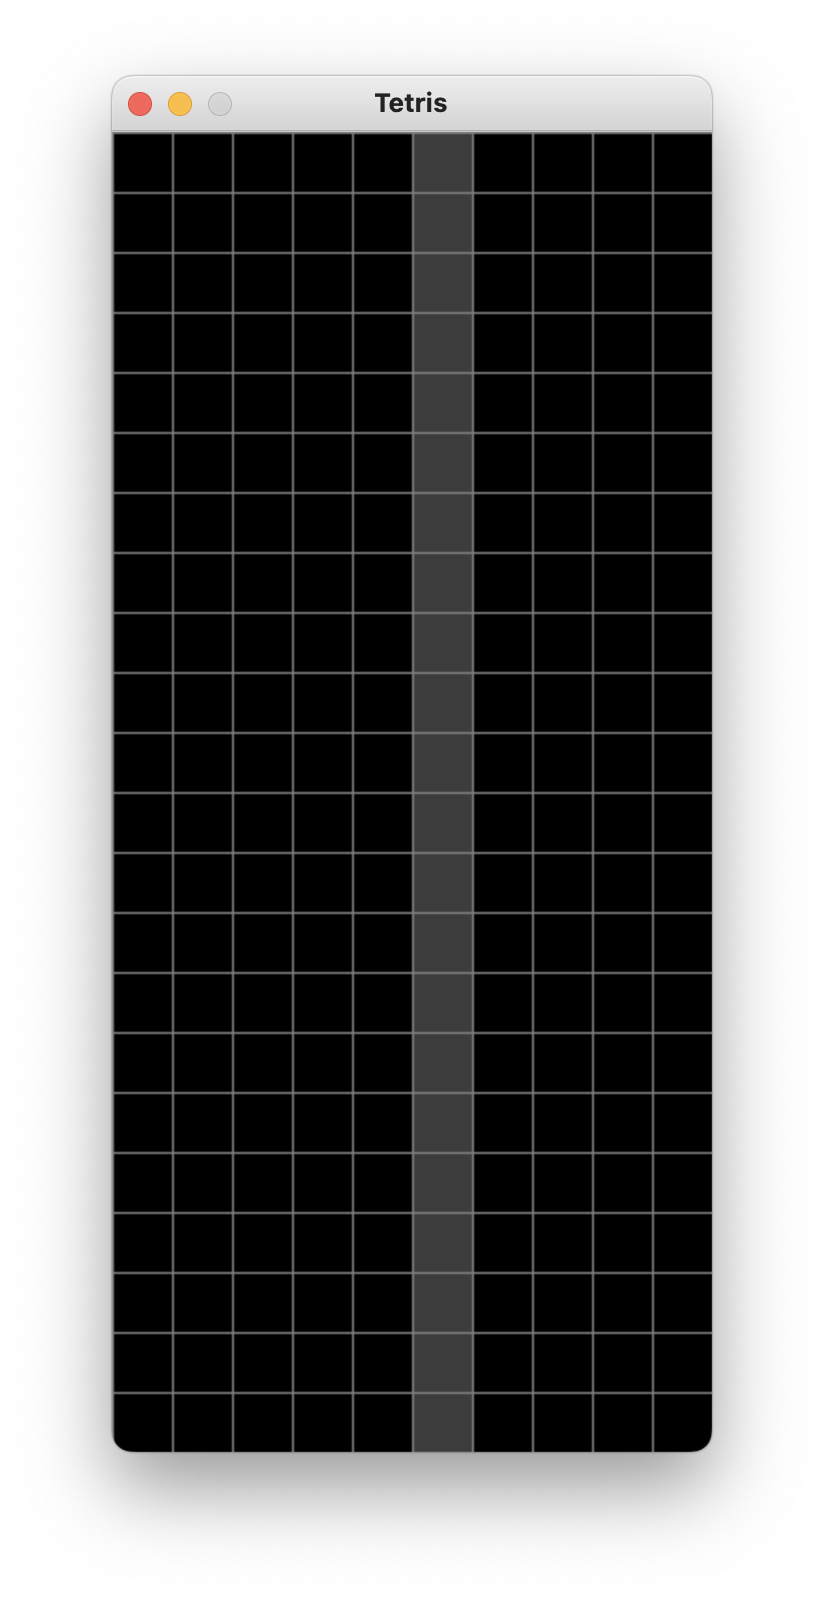
\includegraphics[height=15cm, natwidth=824,natheight=1600]{TetrisCH5.png}
  \caption{テトリスの実行結果}
\end{figure}

\section{カーソルを動かす}
\subsection{キー入力を受け取る}
カーソルを動かすには、キー入力を受け取る必要があります。
さて、画面の話でもありましたが、キー入力を受け取る存在も一つにまとめた方がいいです。
どうやって設計すればいいでしょうか?
\begin{itemize}
  \item キー入力を受け取るクラスを作る
  \item main関数にキー入力を受け取る処理を書く
  \item Boardにキー入力を受け取る処理を書く
  \item Cursorにキー入力を受け取る処理を書く
\end{itemize}
このような方法が浮かんできたら、あなたもオブジェクト指向プログラマーの仲間入りです。

キーを受け取るクラスを作る方法はとても「アリ」なんですが、今回はキーの数が少ないのでしません。
Boardにキー入力を受け取る処理を書くと、Boardがキー入力を受け取るという役割が増えてしまいますし、
そもそも盤面に対してキーを打っているわけではないので、これは残念ながら良くないデザインとされます。
Cursorも同様です。今回は「キー入力を受け取るのはmain関数の仕事」とします。後々一時停止や終了などのキーを
作った時に、それをカーソルが受け取るのは不自然ですよね。

\subsection{main関数でキー入力を受け取る}
先ほど決めた通り、main関数でキー入力を受け取ることにします。
\lstinputlisting[title={main関数でキー入力を受け取る}]{chapter5/main2.py}
矢印キーでカーソルを動かせるようになりました。pygame.time.wait(100)という見慣れない
文があるかもしれませんが、これは100ミリ秒待つという意味です。mb.sleepと似ていますね。

\section{まとめ}
いろいろ考えた結果、今回はカーソルはBoardの一部ということにして、カーソルの描画はBoardに任せることにしました。
さらに、キー入力を受け取るクラスを作ることも考えましたが、今回はmain関数で受け取ることにしました。
このような設計は先を見据えて行うことが重要ですが、慣れないうちは「とりあえず動くもの」を作ることも大事です
\footnote{今回の設計も正しいとは言い切れません。Boardクラスが「Blob(ブロブ)」状態に陥る兆しがあります。詳しく知りたい人は調べたり聞いてみたりしてください。}。

\subsubsection{先生と考えよう}
キー入力を受け取るクラスを作る場合、どのような設計になるでしょうか?

\chapter{テトリスのブロックを作る}
この教材はまだ作成途中です。完成までお待ちください。残りの授業時間はタイピングや
この教材の誤字脱字、わかりにくい箇所を探す時間にしていただけると嬉しいです。

\end{document}